\chapter{Zenithal Hourly Rate Validity for Radio Detection} \label{chap:zhr}
\begin{strip} 
	\begin{minipage}{\textwidth} 
		\begin{abstract} 
	I present an improved formula for calculating Zenithal Hourly Rate (ZHR) and
	an analysis of its validity for radio meteor detection. Beyond this, I
	assess the implications of the resultant ZHR for antenna field of view,
	meteor shower population index and stream density. The formula, with
	modification is valid, and the results agree well with visual results. There
	are clear improvements that can be made, though as a first approximation the
	formula is adequate.  
		\end{abstract} 
	\end{minipage}
\end{strip}

\section{Background} Zenithal Hourly Rate (ZHR) is a measure of the activity of
a meteor shower. The value indicates how many meteors an observer can expect to
see, assuming optimal viewing conditions, with the meteor shower radiant at the
observer's zenith (directly overhead).

\section{Literature Review}

\subsection{Calculating ZHR} A formula already exists for calculating the
theoretical ZHR from known data and conditions \cite{zhr}. The formula
(\ref{eq:zhr}) depends on four correction factors.

\begin{equation}{ZHR} = \frac{\overline{HR} \cdot F \cdot r^{6.5-{m}}}{\sin
\left( h \right)}\label{eq:zhr} \end{equation}

The hourly rate is given by $\overline{HR} = \frac{N}{T_{eff}}$, $N$ is the
number of meteors observed, and $T_{eff}$ is the effective observation time of
the observer. This corrects the number of meteors detected such that it is an
hourly rate. \\ The correction for the field of view, $F$, is given by
$\frac{1}{1-k}$ where k is the percentage of the observer's field of view that
is obstructed. \\ The correction factor for limiting magnitude is given by
$r^{6.5-m}$, where $m$ is the limiting magnitude of the observer. This corrects
the value such that it is representative of the ZHR when the limiting magnitude
is 6.5.  The value of $r$ itself is the population index: a measure of the
magnitude distribution of the shower. For each increase by 1 in magnitude
(bearing in mind that a greater magnitude is a lower value), the number of
meteors you would expect to see increases by $r$.\\ The final correction factor
is for the altitude of the radiant above the horizon, measured as an angle.
This is effectively $\frac{\pi}{2}-z$ where z is the zenith distance in
radians. The radiant is the observed point of origin for all meteors in the
shower. This correction factor is given by $\sin h$ where $h$ is the angle from
the horizon to the radiant.\\

\subsection{Meteor shower information}

The International Meteor Organisation (IMO) provides a list of ``meteor shower
calendars'' \cite{imo_meteor_calendar}. These contain a list of notable meteor
showers, with information on these showers including the active range (period
in which the shower produces visible meteors), the date of its maximum, the
expected ZHR, radiant co-ordinates (in right ascension and declination), and
finally the population index. This calendar will be the source of my data for
visual observation data, and will provide the information from which
comparisons can be made with the radio observation data.

\section{Methodology}

\subsection{Assumptions}

The following assumptions are made in my calculations.  
\begin{itemize} 
	\item The receiving antenna is active for the entire period where data is
	available.  
	\item The antenna detects meteors across the entire sky.  
	\item Detected meteors are travelling tangential to Earth's surface.  
	\item The shower meteors are incident uniformly in all directions around the
		radiant.
\end{itemize}

\subsection{Formula modification}

The formula \cite{zhr} for ZHR has a number of issues that cause inaccurate
results. In order to use the formula in my analysis, these errors must be
corrected.

\subsubsection{Inaccuracy of radiant height correction}

\paragraph{Problems\\} Perhaps the largest error is that of the radiant height
correction. The correction assumes a sine function of the angular radiant
height, which varies (with $-\frac{\pi}{2} \leq h \leq \frac{\pi}{2}$) between
-1 (for $h = -\frac{\pi}{2}$) and 1 (for $h = \frac{\pi}{2}$). This creates a
number of issues: when the radiant approaches the horizon, $h$ approaches 0, as
does $\sin h$. This means that the correction (which is $\frac{1}{\sin h}$)
approaches $\infty$. This is clearly wrong. When the radiant approaches the
horizon, the number of meteors observed doesn't approach 0, and thus the
correction should not approach $\infty$. In other words, you do not see
infinitely many meteors when the radiant is at the zenith compared to the
horizon. Further to this, the use of a sine function simply means that there is
\textit{no} way a calculation can be made when the radiant is at the horizon
--- this should be possible. The sine function also results in a negative ZHR
when the radiant is below the horizon. Clearly, you do not expect to see
anti-meteors when the radiant is below the horizon. 

\paragraph{Previous Solution} Solutions to the issue with the radiant height
correction factor have been studied previously \cite{hr_correction}. In this
article, a piecewise function is noted from Kres\'{a}k \cite{kresak} which uses
a cosine function of the zenith distance (which equates to a sine function of
the radiant altitude) down to 80$^{\circ}$, and then uses another function
which extends the domain of the model to ${\sim}$100$^{\circ}$. The article
itself puts forward a complex function which works over a similar domain. This
is not a first approximation though, it is an attempt at an accurate function
to describe the flux correction factor for a range of radiant altitudes. The
article notes that there is a small, yet present, possibility of shower meteors
for a radiant below the horizon, and the reason for this dramatically lower
expected detection count is that the atmosphere shields the Earth from most of
the debris, and only those travelling tangential to the Earth's surface are
detected. This may be applicable to visual observation, but radio detection
almost relies on meteors travelling tangential to the Earth's surface, so the
radiant being below the horizon does not have such a dramatic effect. For this
reason, I do not believe this is a useful replacement for the correction
factor.

\paragraph{Solution\\} From a basic geometric standpoint, the number of meteors
you expect to observe, varying with the radiant height, should depend on the
proportion of a hemisphere (with the radiant at the pole) that is visible. Of
course, this assumes that meteors travel from the radiant uniformly in all
directions. 

\begin{figure}[h!] 
	\centering 
	\includestandalone[mode=buildnew,width=\linewidth]{wedge} 
	\caption{Spherical wedge curved surface area
	\label{fig:wedge}} 
\end{figure}

A wedge of a sphere has a curved surface area of $2{\alpha}r^2$, where $\alpha$
is the angle at the central axis of the wedge (see figure~\ref{fig:wedge}).
Thus, the proportion, $p$, of the hemisphere that is visible is
$\frac{2{\alpha}r^2}{2{\pi}r^2} = \frac{\alpha}{\pi}$. For an angle $h$ (the
radiant height as an angular distance) varying between $-\frac{\pi}{2}$ and
$\frac{\pi}{2}$, the proportion will vary between -1 and 1 (perhaps where the
original sine factor came from). When the radiant is at the zenith, you would
obviously expect to see the same number as if the radiant was at the zenith, so
the correction factor, $c$, is 1 (see figure~\ref{fig:hemisphere}). 

\begin{figure}[h!] 
	\centering 
	\includestandalone[mode=buildnew, width=\linewidth]{diagram} 
	\caption{Diagram for derivation of radiant height correction factor. The
	shaded hemisphere is the observer's field of view.}
	\label{fig:hemisphere}
\end{figure}

When the radiant is at the horizon, half the hemisphere is visible, so you
would expect to see half the number of meteors at the zenith ($c = 2$), and
when the radiant is directly below you (at the nadir) then you would expect to
see no meteors (from the shower), since none of the hemisphere of the radiant
is visible to you. Mapping the proportion linearly from $-1 < p \leq 1$ to $0 <
\frac{1}{c} \leq 1$ yields $\frac{1}{c} = \frac{1}{2} + \frac{h}{\pi}$ for
$-\frac{\pi}{2} < h \leq \frac{\pi}{2}$, where $h$ is in radians. This
satisfies the \textit{expected} correction factor.

\subsubsection{Population index limitations}

The population index indicates the magnitude distribution of the meteor shower.
For each extra magnitude of visibility, an observer would expect to see $r$
times more meteors. This is true, but only up to a point. Without a limit on
how far this model works, the implication is that this power-law distribution
carries on forever. Clearly this is not true: if limiting magnitude was (rather
absurdly) 40, you wouldn't expect to see 1.1 trillion meteors (if $r=2.0$).
Thus the model is not applicable for limiting magnitude, $m > 6.5$, since the
model that the magnitude distribution is of the form $N = N_or^m$ is no longer
valid. The radio observation of meteors has a larger limiting magnitude than
visual observation: meteors down to the size of a grain of sand, and smaller,
can be detected. Thus the population index model is not applicable for radio
meteor detection, unless the model is refined for larger limiting magnitudes.

\subsubsection{Background detection count}

In visual observation of meteors, the background level of sporadic meteors is
rather low. However, for radio meteor detection, there is a much greater
background detection rate and this will impact how accurate the ZHR is. A
correction is required to remove the effect of any background detection rates.
The calculation of this background rate is a chapter in itself. If the baseline
is larger than any detection counts within the active range, the resulting ZHR
will be negative, and this is not a valid result. A solution to this is to
choose the minimum hourly detection count in the active range of the shower,
but this is rather artificial, and often results in a baseline of 1 or 0.
Instead, I have decided to calculate the background hourly detection count by
taking the mean hourly detection count for the lower quartile of all hours
outside the active range of any meteor showers. This will result in some ZHRs
being negative, but these results should be minimal and can simply be
discarded.

\subsubsection{Field of view correction}

I will not include a field of view correction factor, since it is not possible
to know exactly the field of view that each antenna has available, because it
is not part of any data that an observer can upload to RMOB. This
\textit{should} have a reasonably large impact on the results, however the
correction factor will be absent for all calculations so the error is the same
everywhere (on average). In fact, the final results may allow the average field
of view to be calculated.

\subsection{Calculating radiant height}

From the spherical law of cosines, we know that
\[ \cos z =  \sin \phi \sin \delta + \cos \phi \cos \delta \cos \left( \theta -\alpha \right)\] 
where $z$ is the zenith distance, $\phi$ is the observer's latitude, $\alpha$
and $\delta$ are the right ascension and declination of the shower radiant, and
$\theta$ is the local apparent hour angle (an angular measure of local sidereal
time, which effectively measures time against the stars rather than the Earth's
rotation).  Since $h = \frac{\pi}{2} - z$, $\cos z$ can be replaced with $\sin
h$. This relates the radiant altitude to the longitude of the observer and the
radiant's astronomical co-ordinates.

\subsection{Calculating hourly rate}

The hourly rate is given by the observed hourly rate (the data I actually
have), minus the baseline hourly rate. This \textit{should} be divided by the
effective observation time, but since I am making the assumption that the
antenna are receiving across the entire hour, then there is no need for this.

\subsection{Analysis}

\paragraph{Selecting observers}

In order to carry out the analyses, the observers had to be split into groups
for each shower. This was done simply by checking which months each observer
was active for, and adding it to a given category if the observer was active
during the shower. This selection was refined further so that an observer must
be active for the entire peak date, and have no more than 12 inactive hours
during the active period of the shower. The sample sizes for each shower are
shown in table~\ref{tab:zhr:sizes}.

\begin{table} 
	\centering 
	\begin{tabular}{cc} 
		\hline 
		Shower & N$^{\circ}$ observers \\ \hline 
		Geminids & 67 \\ 
		Leonids & 61 \\ 
		Orionids & 43 \\ 
		Perseids & 39 \\ 
		Quadrantids & 58 \\ 
		$\eta$ aquariids & 34 \\ \hline 
	\end{tabular} 
	\caption{Sample sizes for meteor showers \label{tab:zhr:sizes}}
\end{table}

\paragraph{Comparison\\}

My analysis of the ZHR will centre around a comparison between the summary
statistics for the ZHRs from the hourly counts for the stored observers, and
known values for the ZHRs for applicable years. The process of calculating the
ZHR follows a simple process of calculating the correction factors, correcting
the known hourly rate, and discarding any invalid values (e.g. negatives). The
formula, after modification, is
\[ {ZHR} = \frac{N - r}{\left( \frac{1}{2} + \frac{h}{2\pi} \right)} \] 
where $r$ is the background hourly rate, and $N$ is
the number of meteors detected for one hour. The error is given by 
\[ {S.E.} = \frac{{ZHR}}{\sqrt{N}}\] 
This calculation will be done for each hour available,
and then a mean will be taken. This process will be applied to three ranges of
dates: the entire active period of the shower (for a given year), two days
either side of the peak date, and the peak date. Once this has been calculated
for all the available data in the given ranges, the mean and 90th percentile
are recorded. These will then be compared to the known values from the IMO
meteor shower calendar \cite{imo_meteor_calendar}. I am using the 90th
percentile rather than the maximum ZHR since the maximum itself is of little
worth to indicate the distribution of ZHRs. A box plot for each year of each
shower would yield the most information but would provide far too much data to
consider at once, whereas the 90th percentile indicates the maximum clearly
without producing the exact same result if, for instance, the maximum ZHR was
the same across all three periods under consideration. 

In order to assess the agreement between radio and visual ZHR, I use Pearson's
Moment Correlation Coefficient (PMCC) to give a quantitative measure of
correlation, indicating how well radio results reflect visual results.

\paragraph{Correction factors\\}

The final results will then be used to estimate the average field of view
across all observers whose data are used, as well as the average limiting
magnitude. This is a rough calculation, and is likely to have a large
uncertainty, but it gives an estimate towards the true values and is an
interesting calculation to make. The formula for the field of view factor is

\[ k = 1 - \frac{{ZHR}_{mean}}{{ZHR}_{exp}} \]

For the limiting magnitude,

\[ m =  \log_r \frac{r^{6.5} \cdot {ZHR}_{mean}}{{ZHR}_{exp}} \]

For each of these calculations, $ZHR_{mean}$ is the calculated mean ZHR for the
peak of the shower, and $ZHR_{exp}$ is the maximum visual ZHR for the same
shower and year.  It is clear that a negative $k$ will be the result when the
mean ZHR of the peak is less than expected, and positive otherwise. Any
negative values can be discarded. Equally, a limiting magnitude will be less
than 6.5 if the mean ZHR of the peak is less than expected, otherwise it will
be larger than 6.5. Values less than 6.5 can be discarded. This means that the
correction factor that applies will either be for field of view, or limiting
magnitude, not both.

\section{Results}

The full results are shown in appendix~\ref{app:zhr}. In this section,
important results are noted. In graphs comparing radio and visual ZHRs, the
results considering only the peak (indicated by a dot-dash line) are the most
important to consider, since these are for the same period as the maximum visual
ZHR results.

\subsection{Comparison}

\paragraph{Geminids\\}

Figure~\ref{fig:zhr:gem} shows the mean radio ZHRs for the peak period, peak
$\pm$ 2 days, and the entire active range compared to the maximum visual ZHRs
for each year. There is no clear agreement between the two methods of assessing
ZHR.  The results for radio ZHR are lower than expected for all years other than
2012. However,  given the radio ZHRs were adjusted by a certain offset, they may
appear similar to the visual results.

\begin{figure}[h!] 
	\centering
	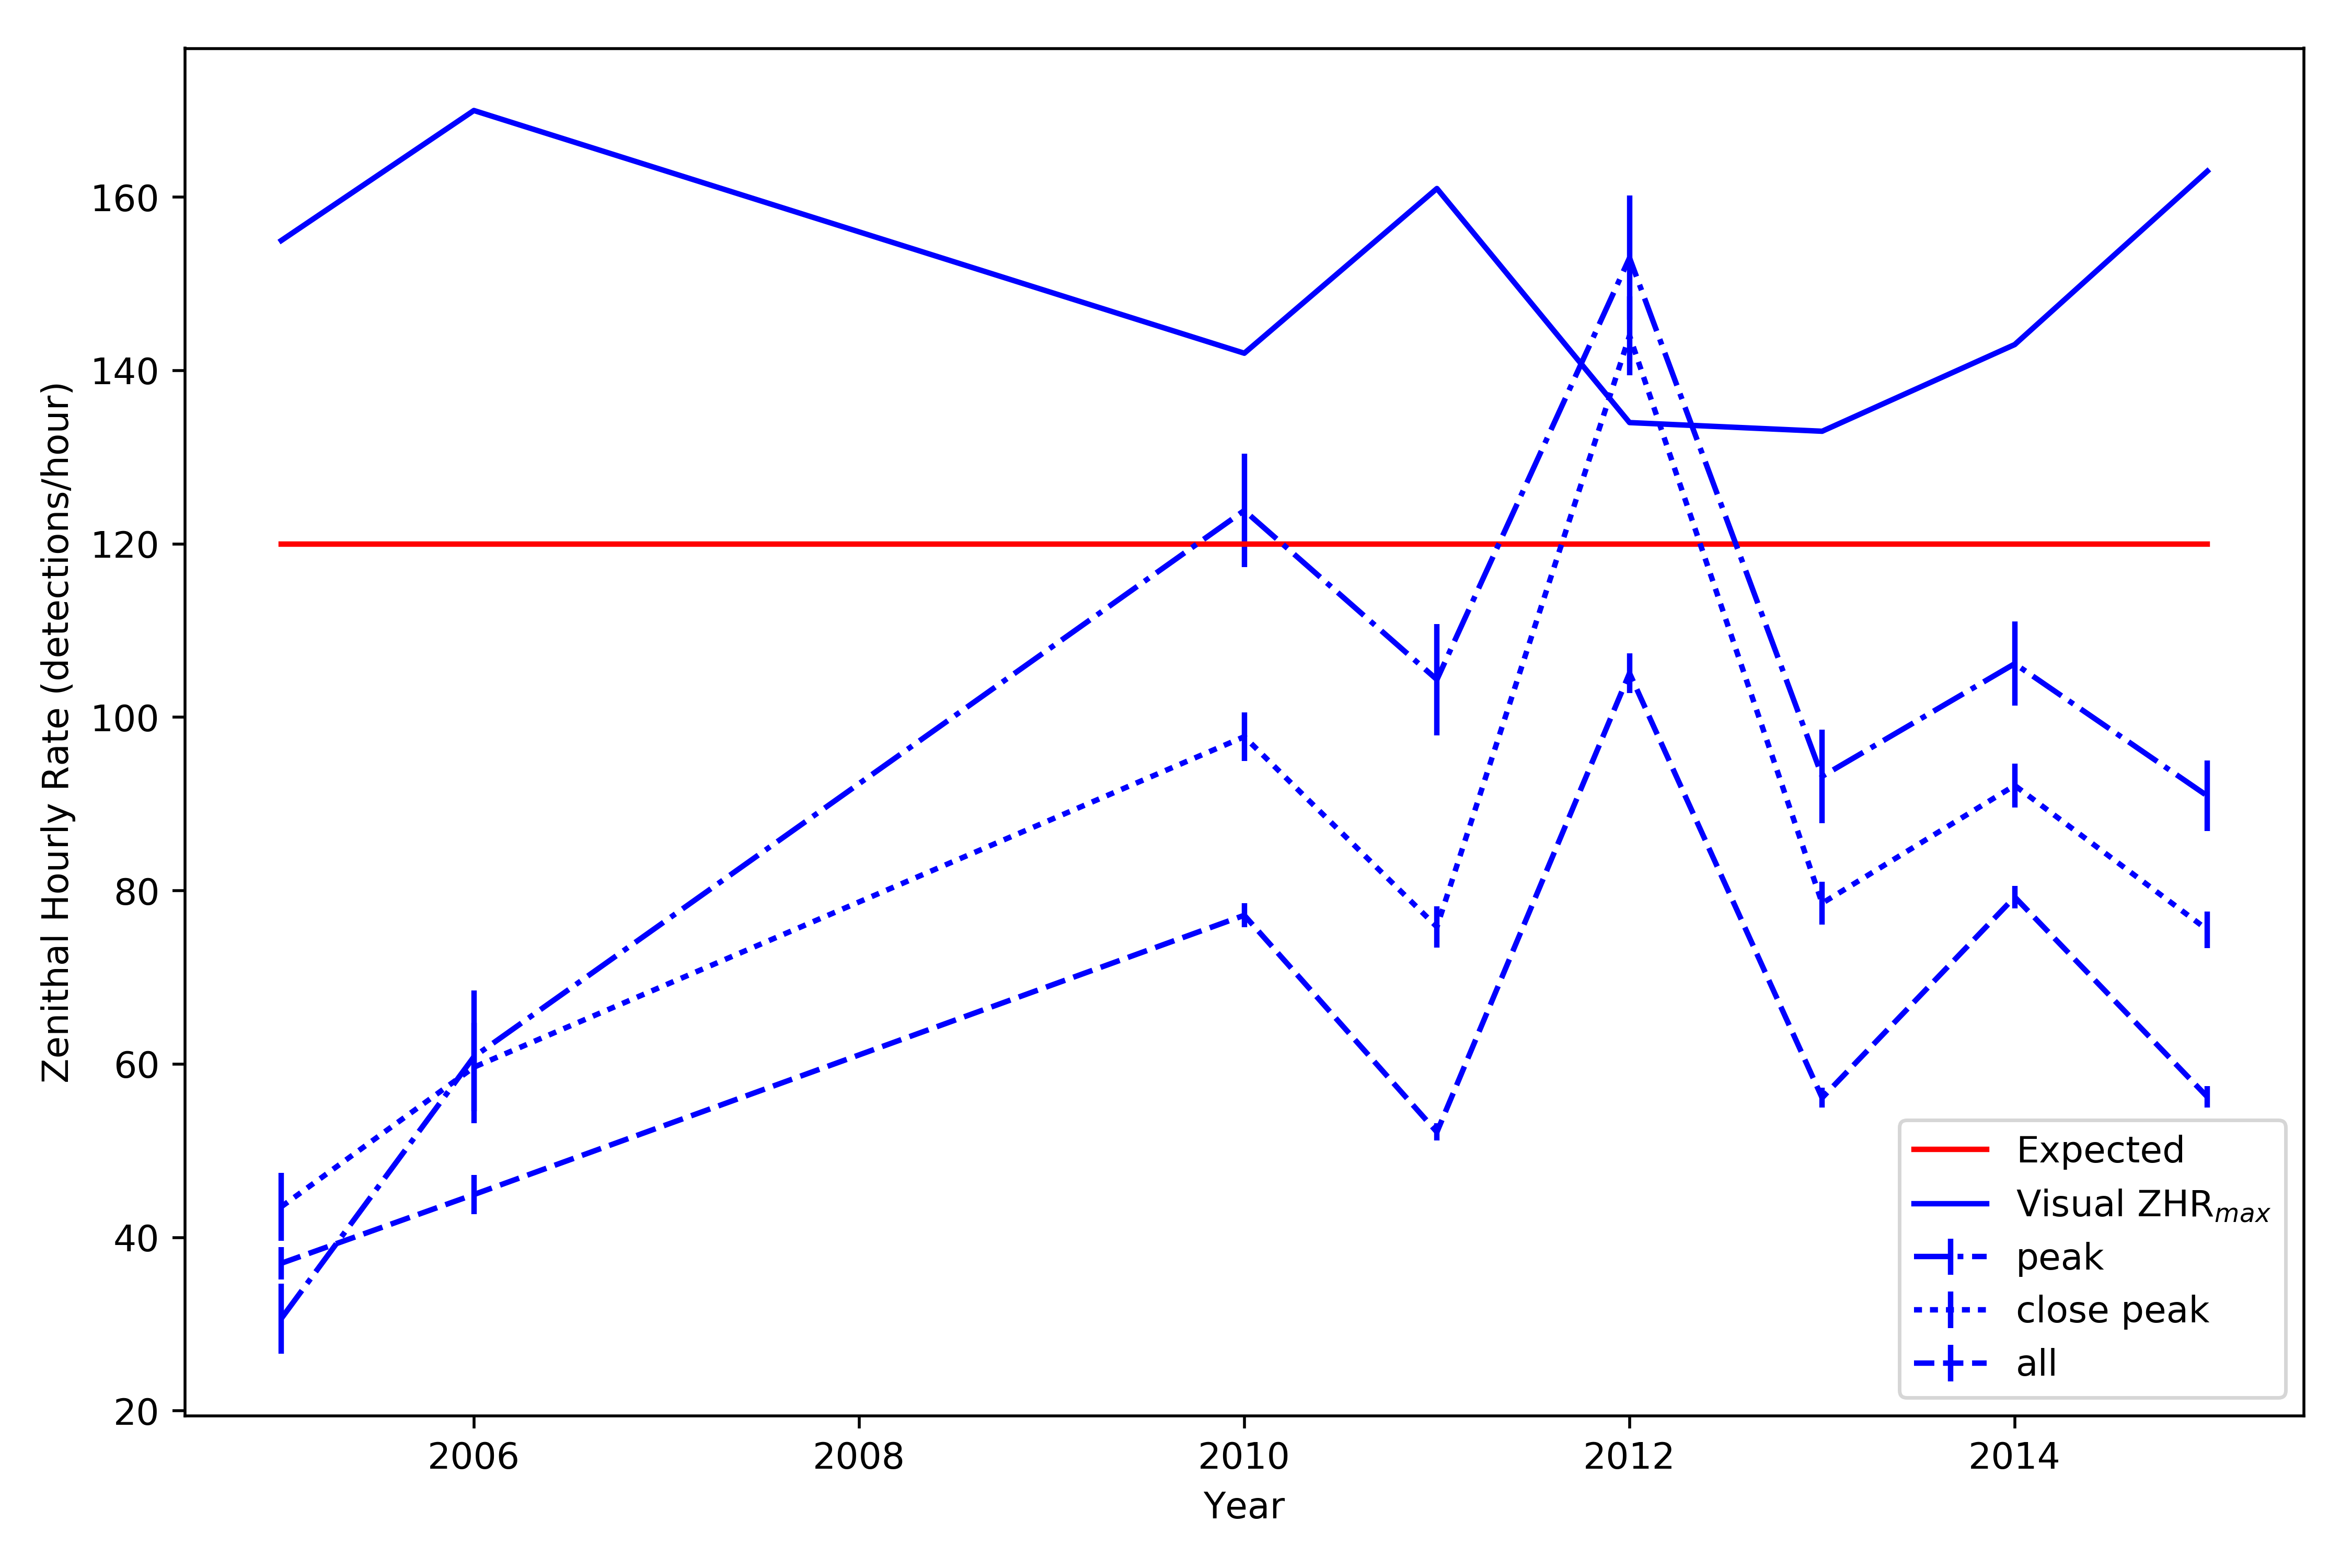
\includegraphics[width=\linewidth]{zhr/geminids_notitle} 
	\caption{Geminids shower mean radio ZHR compared to visual maximum ZHR and
	expected ZHR.} \label{fig:zhr:gem}	
\end{figure}

It is important to note that the radio ZHRs are not dramatically different to
the visual results. The visual ZHRs do not fluctuate more than around 20
detections an hour, and the radio results, whilst fluctuating more than the
visual ZHRs, centre around a certain value in a similar way to the visual
results.

\paragraph{Leonids\\}

The results for 2007 are much higher than expected. Other than this year, the
results are much closer to the visual ZHRs.  The visual ZHRs fluctuate over a
range of ${\sim}20$, and (disregarding 2012) the radio ZHRs appear similar. A
decrease is exhibited in the visual results towards 2016, and this is reflected
in the radio results, indicating good agreement. Equally, the visual ZHR is
lower in 2005 and this is seen in the radio ZHR, too. 2012 stands out as an
erroneous year, though there is a much larger standard error in the results
(indicated by the error bars), suggesting either a low sample size or anomalous
results.

\begin{figure}[h!] 
	\centering
	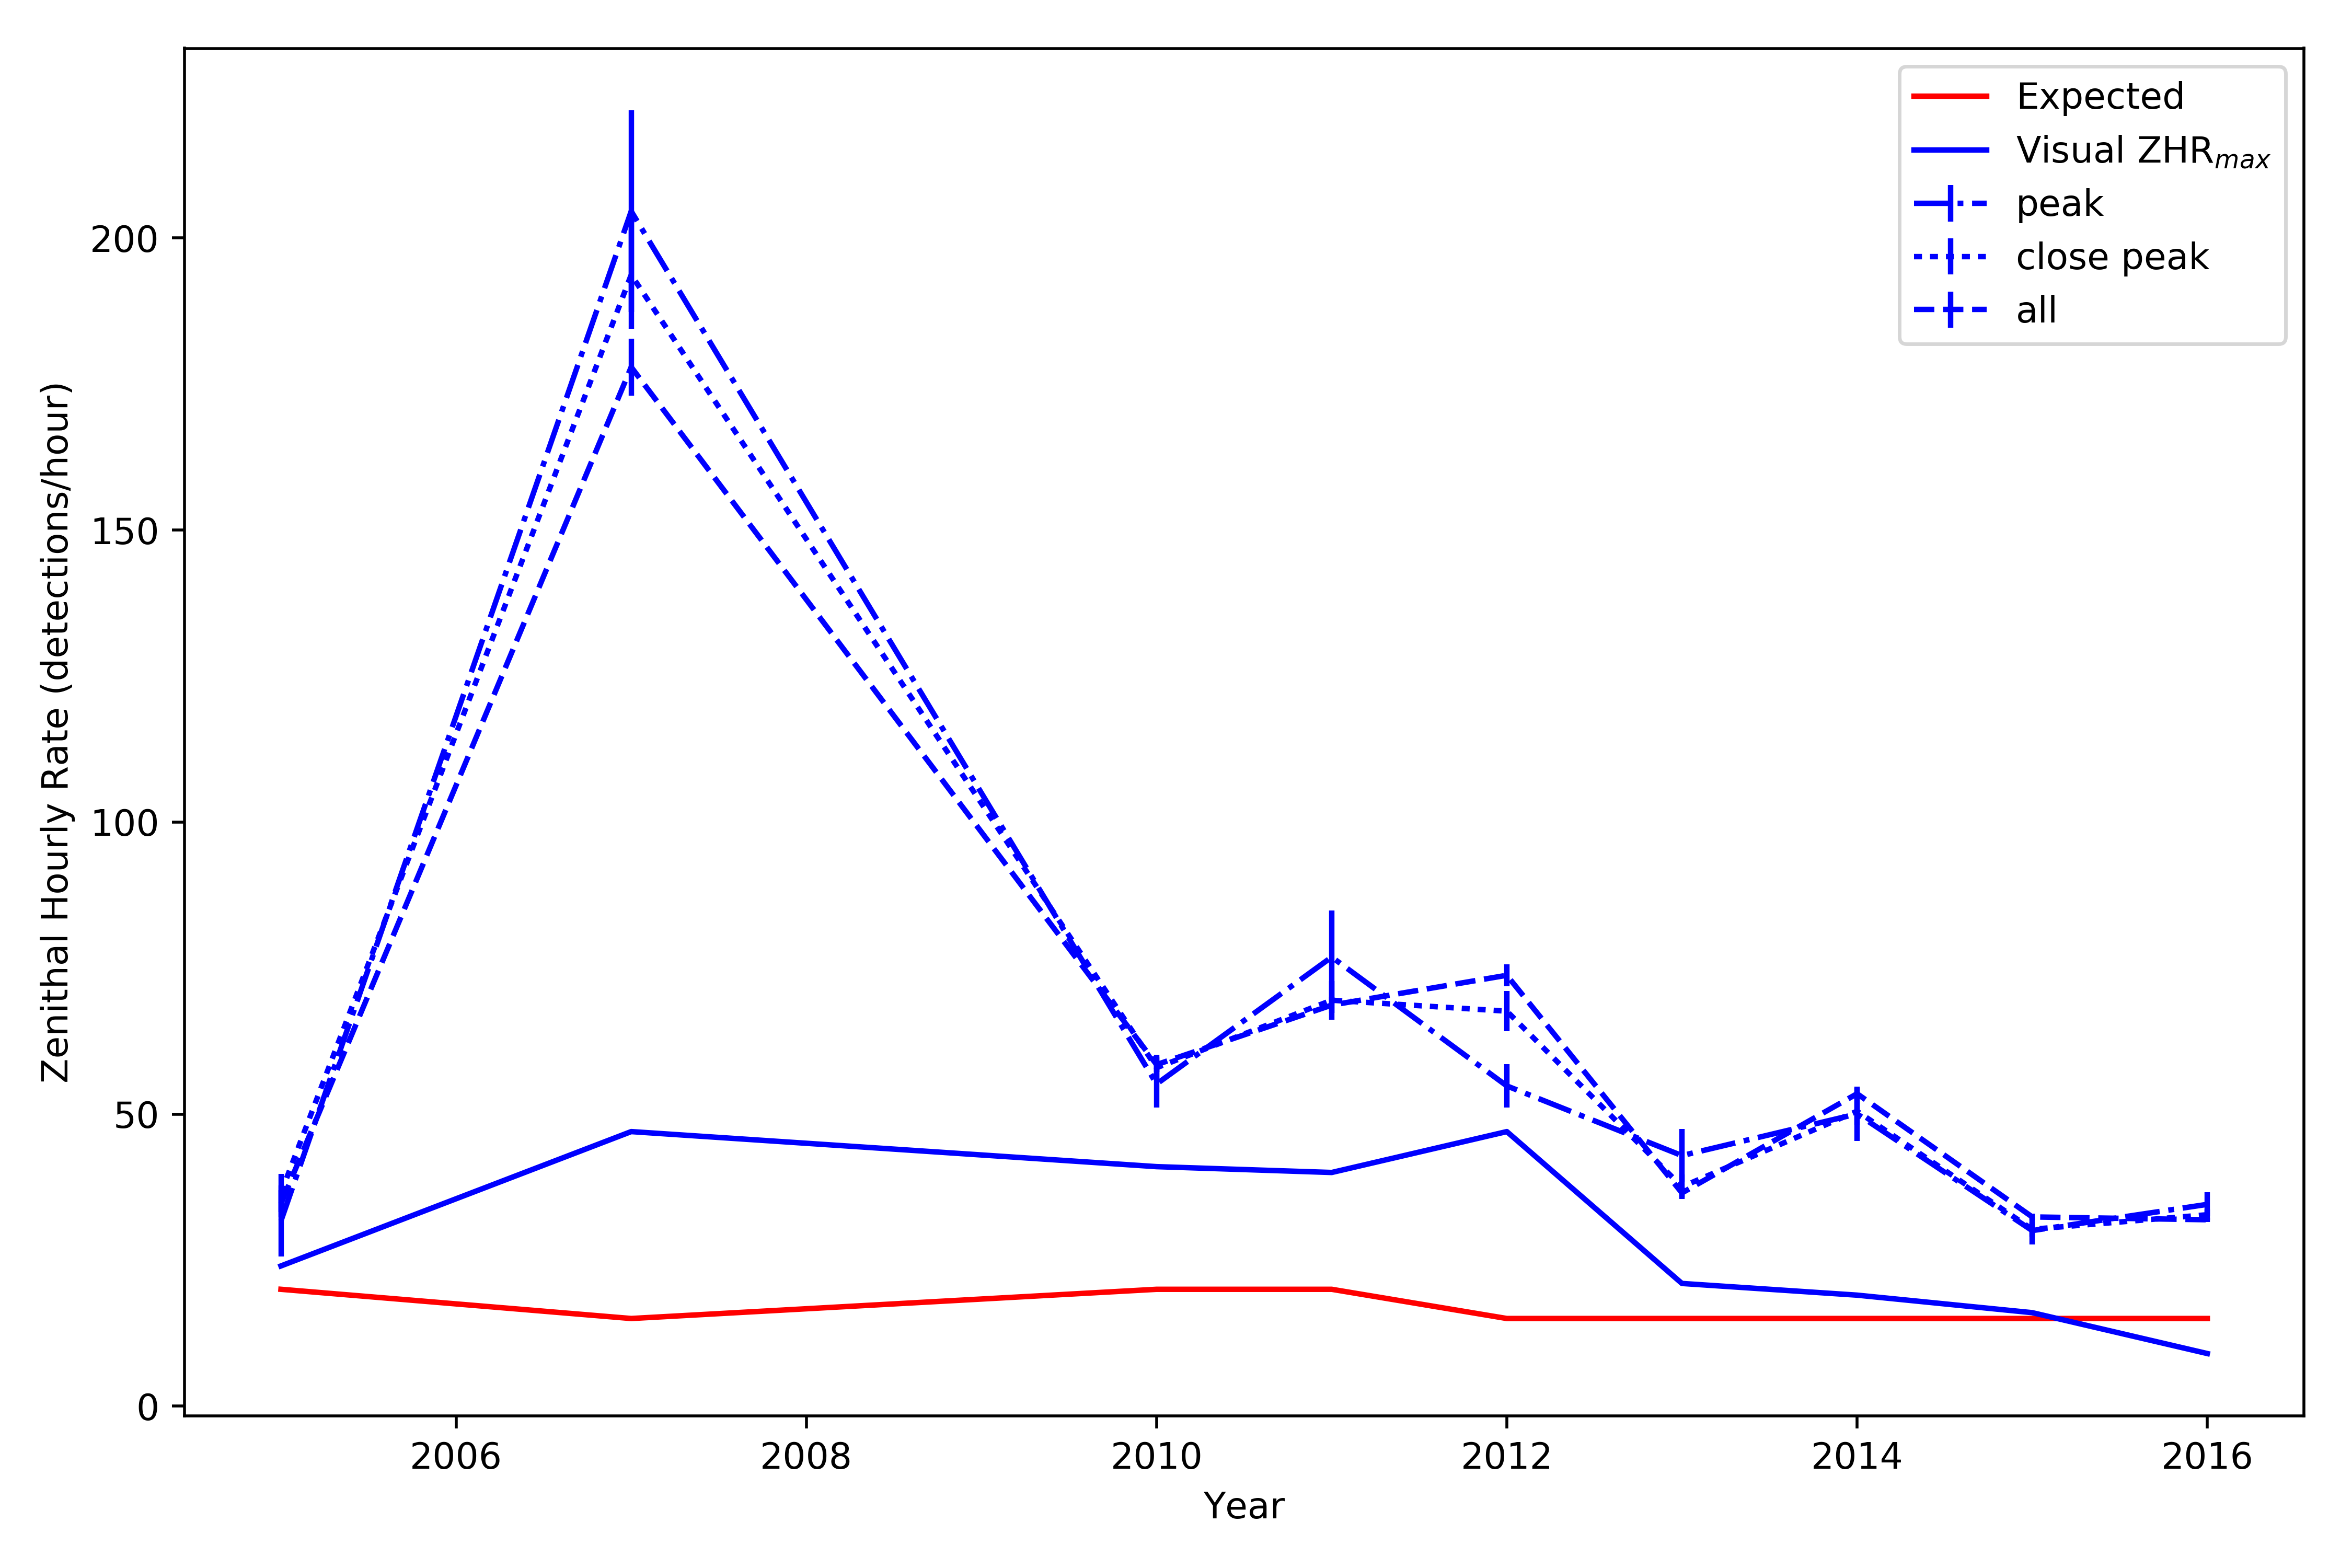
\includegraphics[width=\linewidth]{zhr/leonids_notitle} 
	\caption{Leonids shower mean radio ZHR compared to visual maximum ZHR and
	expected ZHR.}
	\label{fig:zhr:leo}	
\end{figure}

The radio ZHRs are similar to the visual maxima though are greater, however the
correlation between increase and decrease of the expected ZHRs and calculated
ZHRs implies that the issue is simply a matter of a correction factor, e.g.
field of view or population index (the leonid shower may have a large population
index, indicating that with the higher limiting magnitude for radio observation,
you detect more meteors).

\paragraph{Orionids\\}

For all years where data is available, the calculated ZHRs are consistently
greater than expected. However, the radio ZHRs follow a very similar form to the
visual results: the results are larger in 2010 and 2011, decreasing in 2012 and
2013, followed by a slight increase up to 2016. The two sets of data agree with
each other well.

\begin{figure}[h!] 
	\centering
	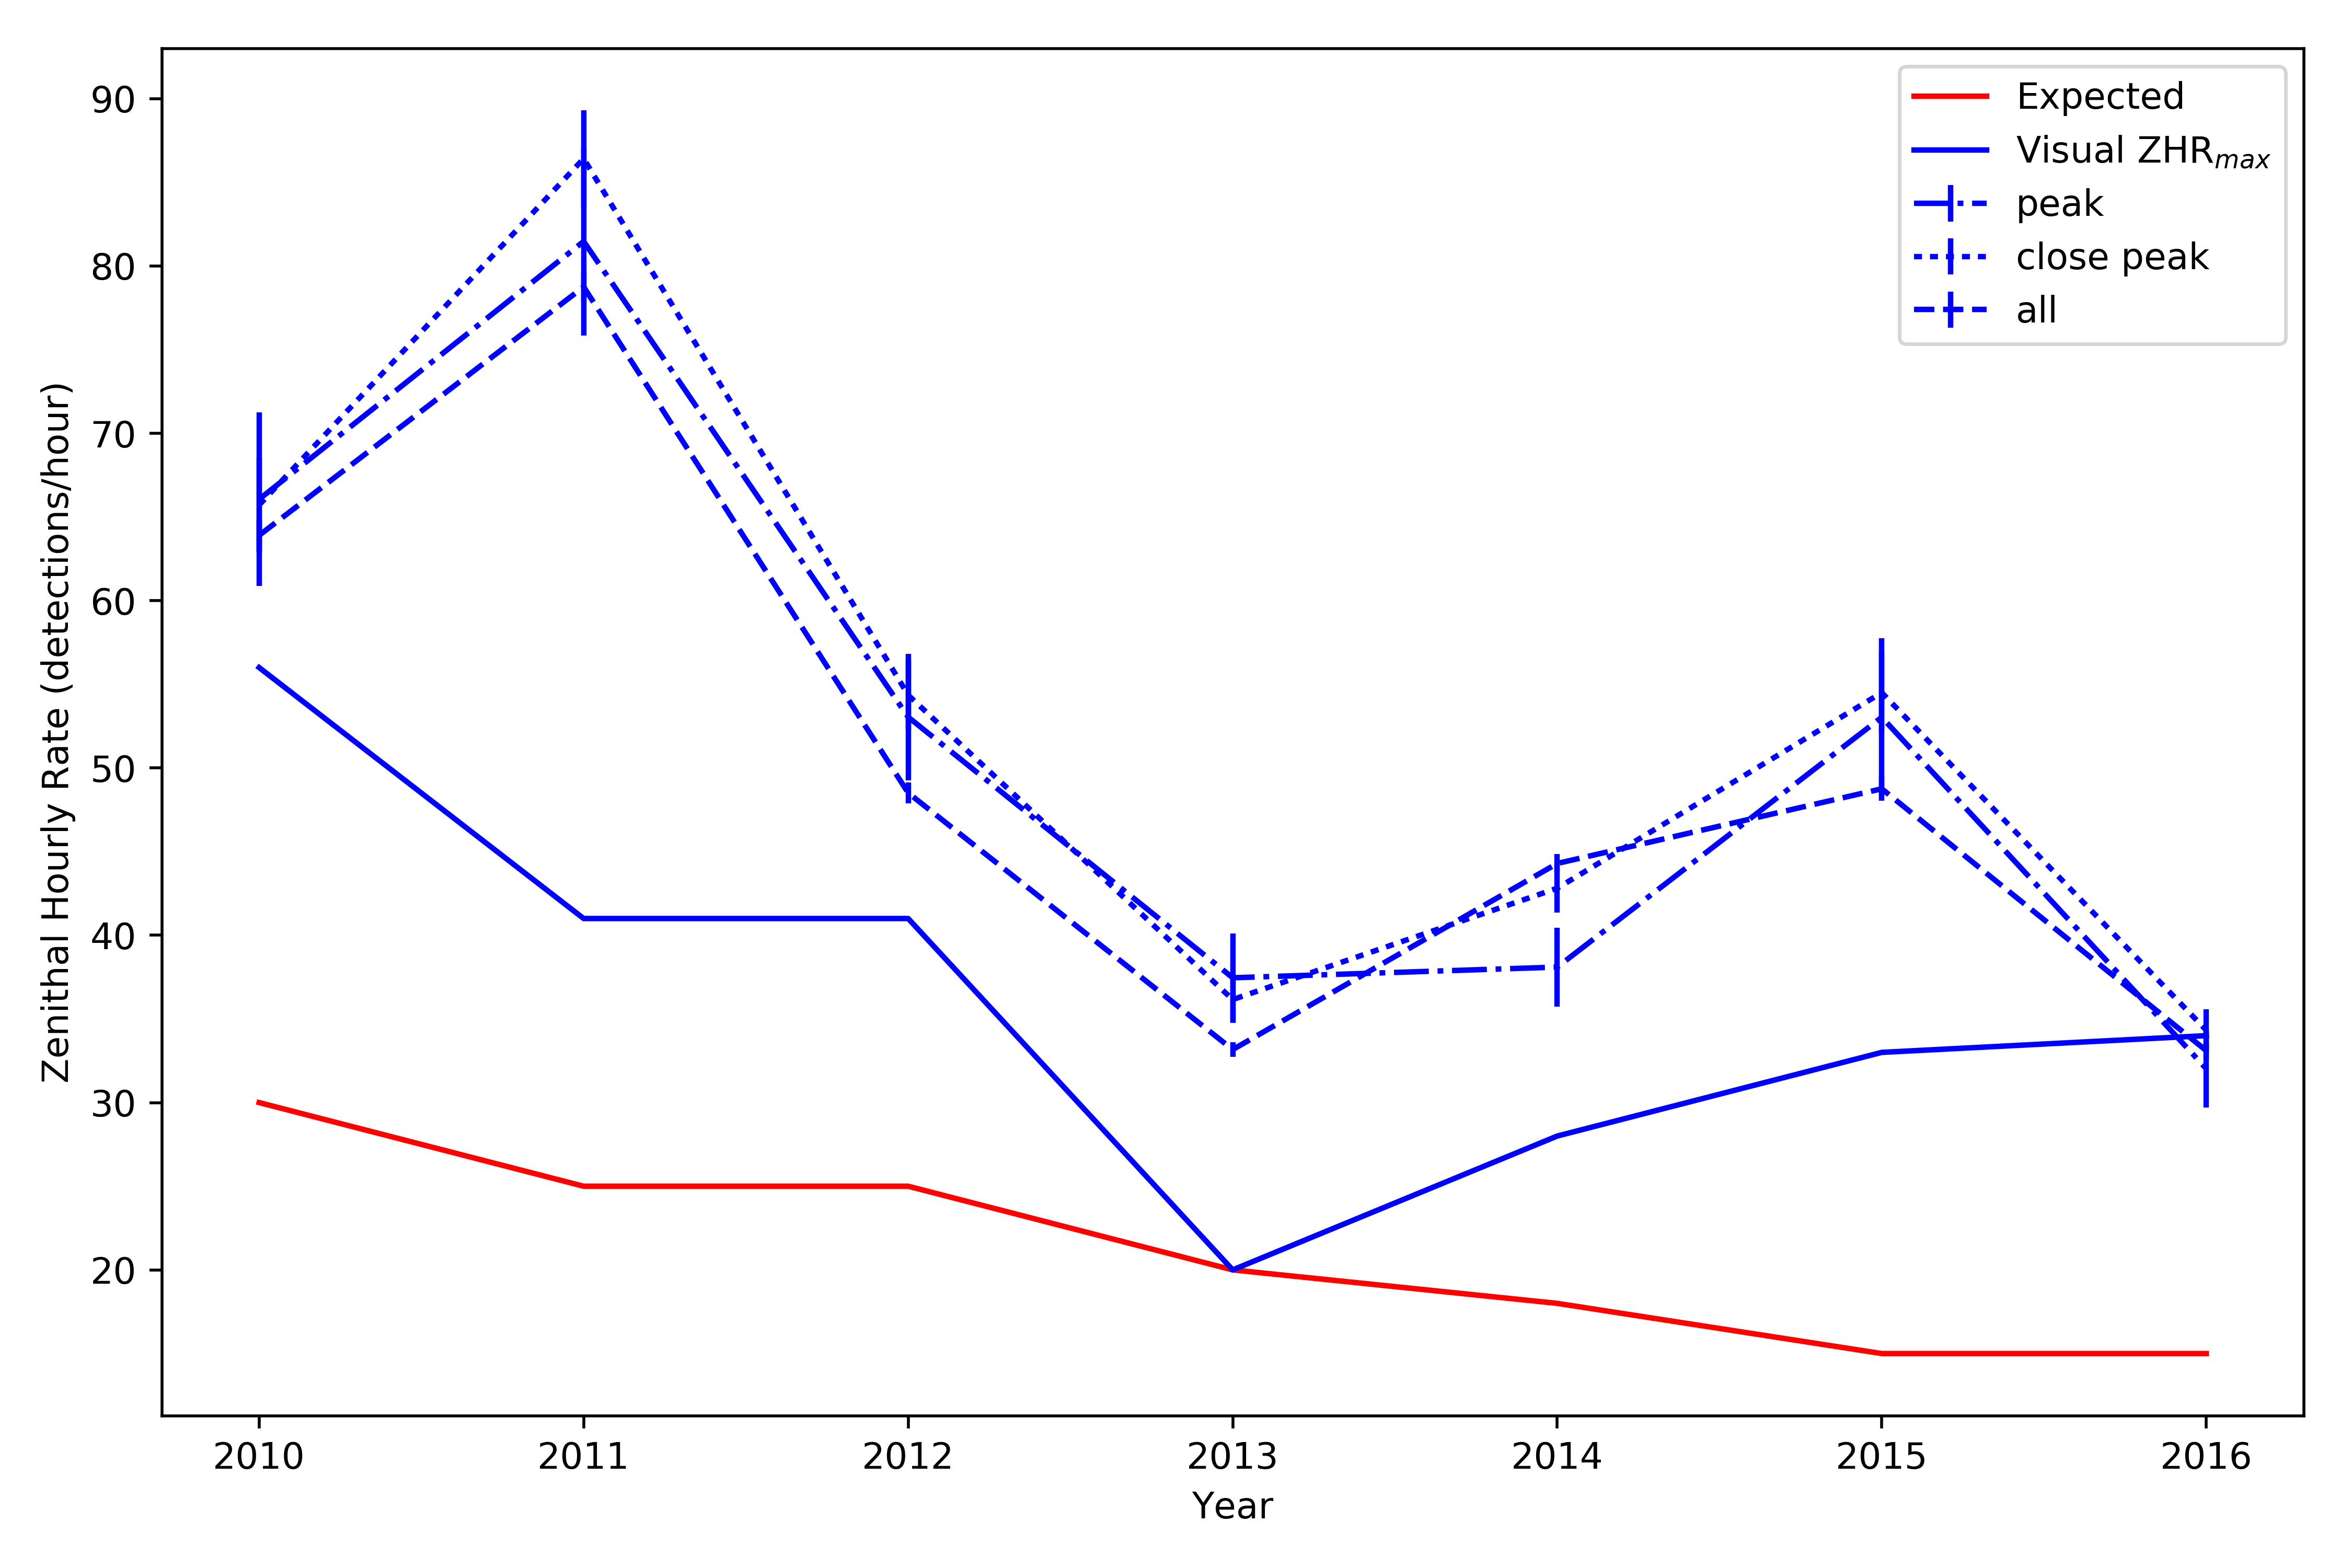
\includegraphics[width=\linewidth]{zhr/orionids_notitle} 
	\caption{Orionids shower mean radio ZHR compared to visual maximum ZHR and
	expected ZHR.}
	\label{fig:zhr:ori}	
\end{figure}

The errors are similar for the considered years. This indicates a good agreement
between the authors in the sample, which in conjunction with the similar forms
indicates that the radio ZHR is a good reflection of visual ZHR. However, the
radio results are consistently greater than the visual results. 

\paragraph{Perseids\\}

Year on year, similar results are seen. The radio and visual ZHRs are similar
for the peak period throughout the years considered. A similar form is seen
between radio and visual ZHRs. In 2010 a larger maximum visual ZHR is recorded,
and the radio ZHR is larger, too. However, not as great as 2012, despite a lower
visual ZHR. Anomalies like this are to be expected, and the more important
detail of form appears to have good agreement between radio and visual. The
maximum visual ZHRs are greater in 2012, 2013, 2015 and 2016, and this is
reflected in the radio ZHRs, other than in 2016. Again, anomalous results such
as this should be expected.

\begin{figure}[h!] 
	\centering
	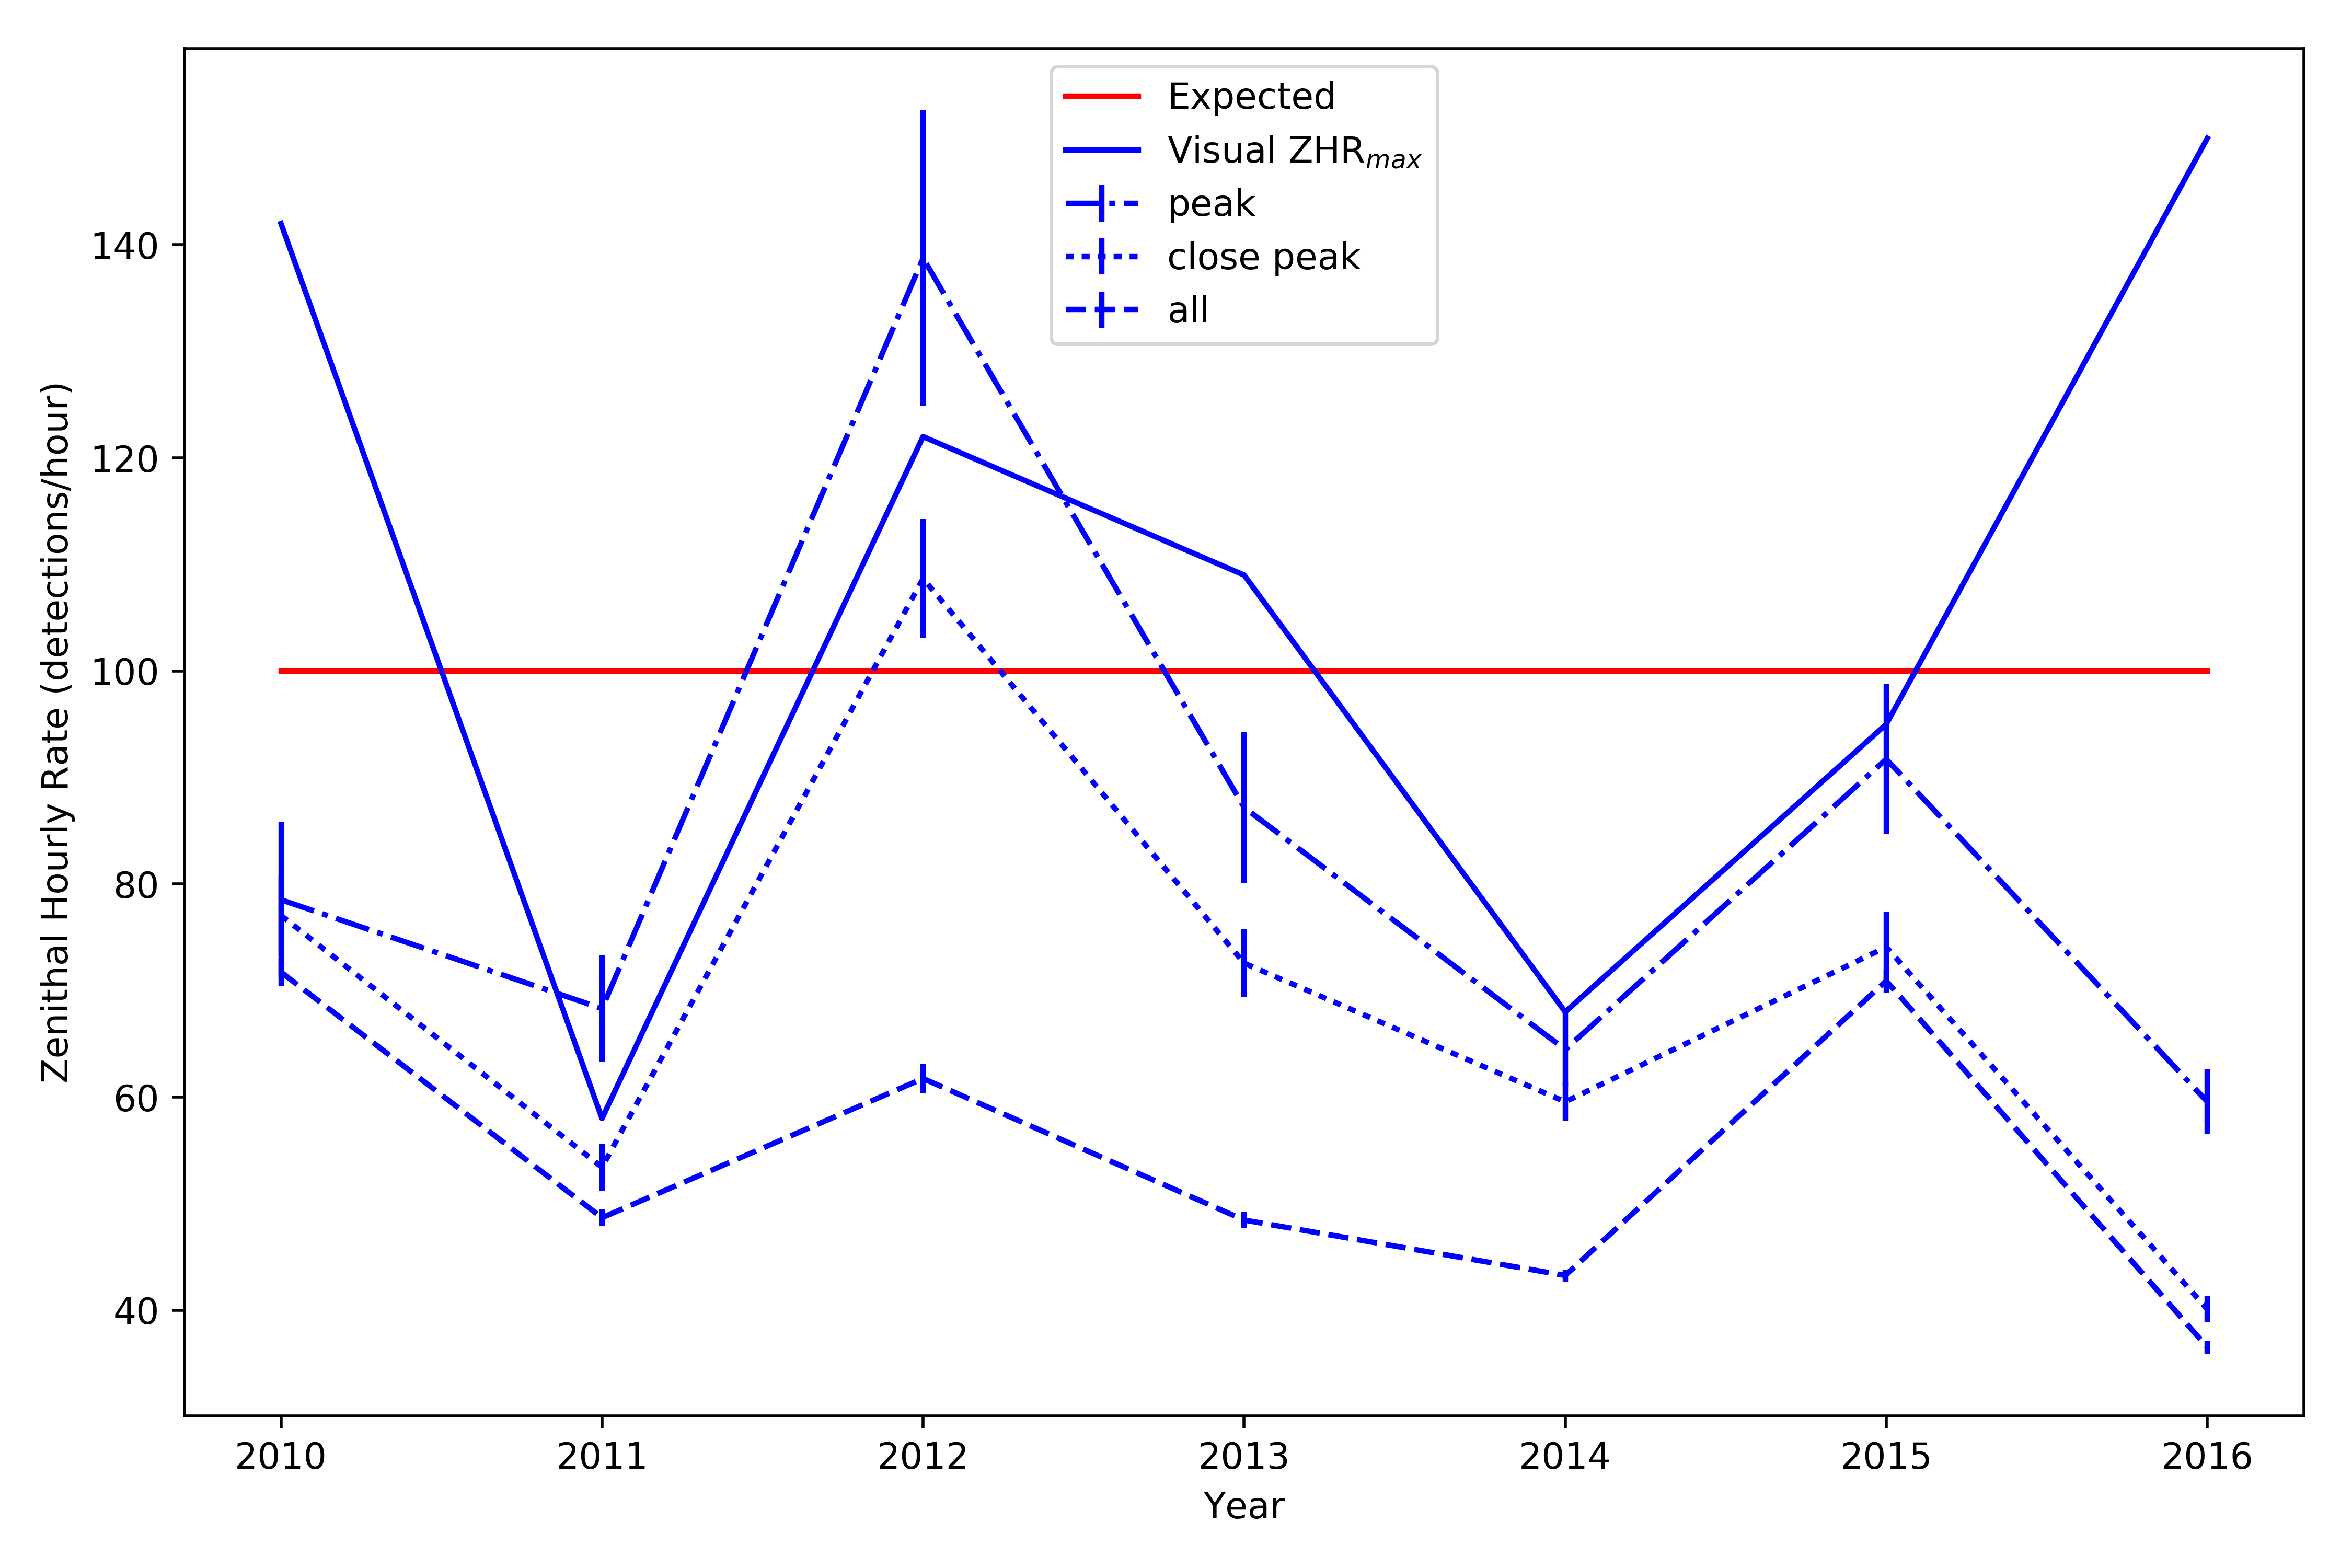
\includegraphics[width=\linewidth]{zhr/perseids_notitle} 
	\caption{Perseids shower mean radio ZHR compared to visual maximum ZHR and
	expected ZHR.}
	\label{fig:zhr:per}	
\end{figure}

Overall, the agrement between the radio and visual ZHRS for the perseid shower
is good. The increases and decreases in visual ZHR between each year are well
represented by the radio ZHR results.

\paragraph{Quadrantids\\}

The variation in the maximum visual ZHRs is reflected well in the radio ZHR
results. In 2011 and 2012 the means for the peak are very close to the visual
maximum. Whilst the remaining years are not as close to the visual maxima, where
the maximum increases (2013, 2014), the mean ZHR for the peak increases, and
then decreases for 2015 and 2016, as does the visual maximum.

\begin{figure}[h!] 
	\centering
	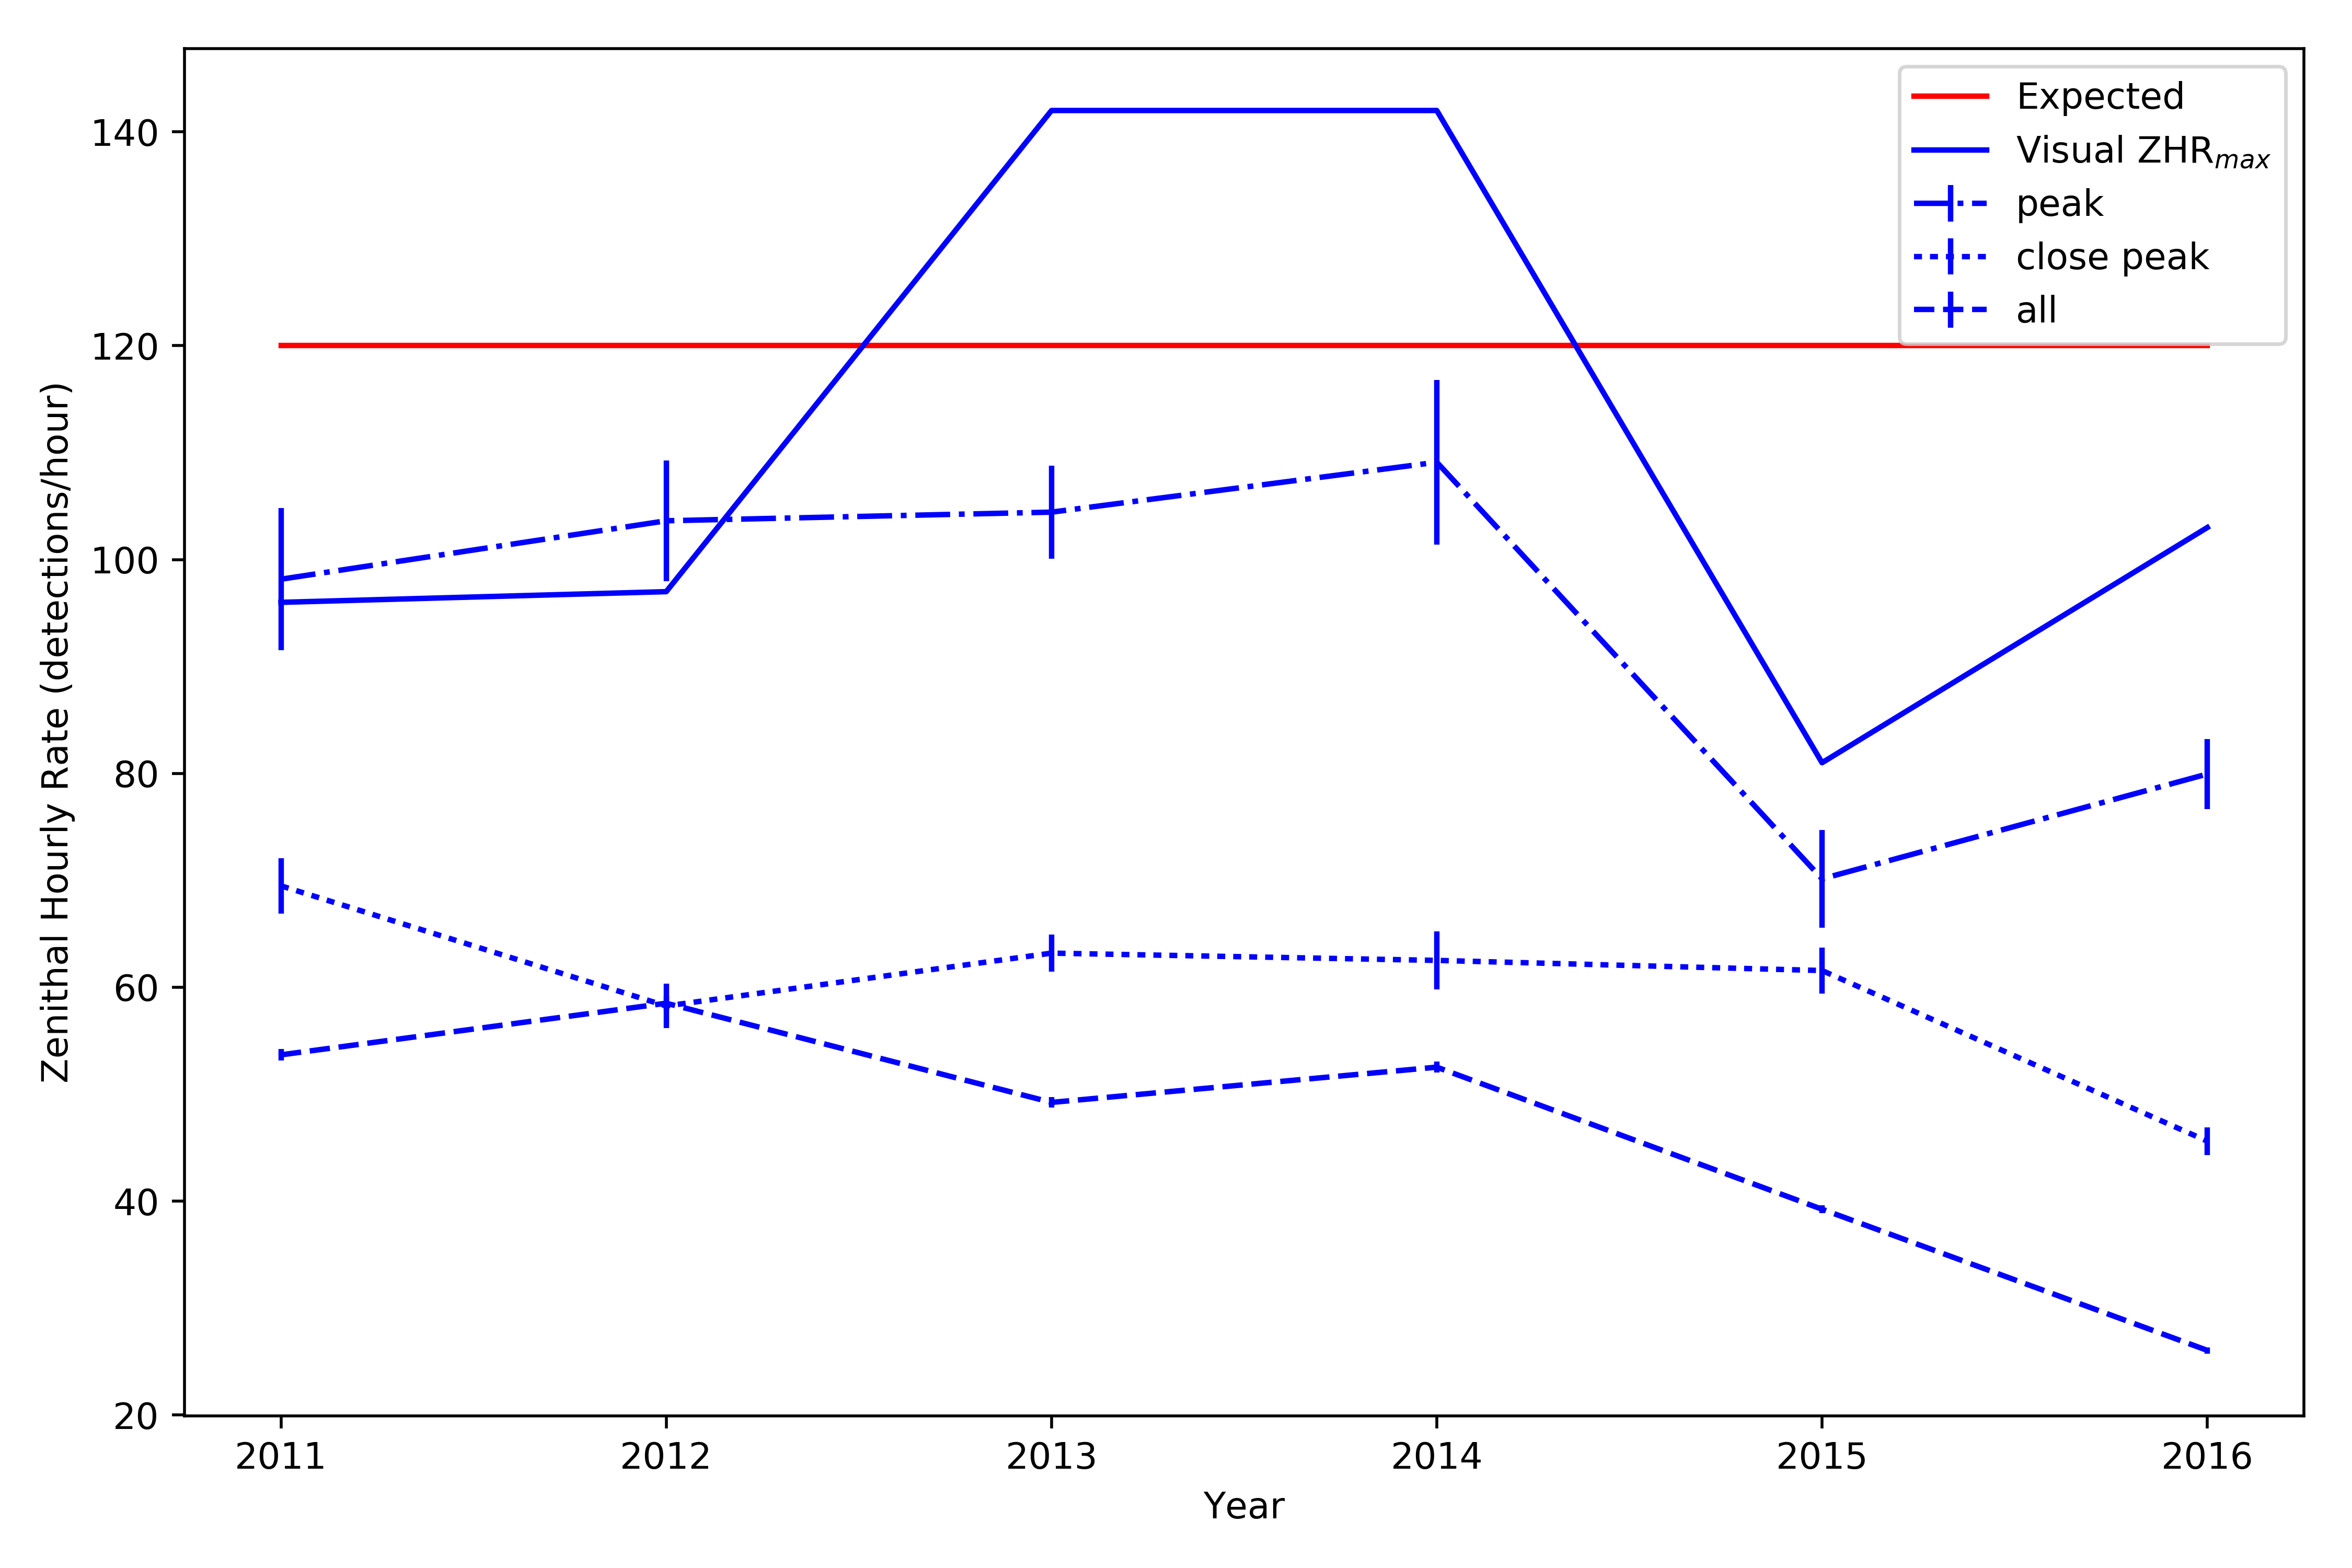
\includegraphics[width=\linewidth]{zhr/quadrantids_notitle} 
	\caption{Quadrantids shower mean radio ZHR compared to visual maximum ZHR
	and expected ZHR.}
	\label{fig:zhr:qua}	
\end{figure}

The results for the peak $\pm$ 2 days, as well as the entire active period are
much lower than the peak period. This change is not seen as clearly for the
other showers that have been analysed. Not only do the results reflect the
visual results well in form, but in value too. The majority of results for
the radio ZHR on the peak day is similar to the maximum visual ZHRs.

\paragraph{$\eta$-aquariids\\}

The results for radio ZHR match those for visual ZHR well. The maximum visual
ZHR decreases from 2010 to 2012, and continue this trend at a lower rate to
2016, other than an anomalous result in 2013 which is much greater than other
years. This trend is matched similarly by the radio ZHRs, other than the
anomalous increase in 2013. 

\begin{figure}[h!] 
	\centering
	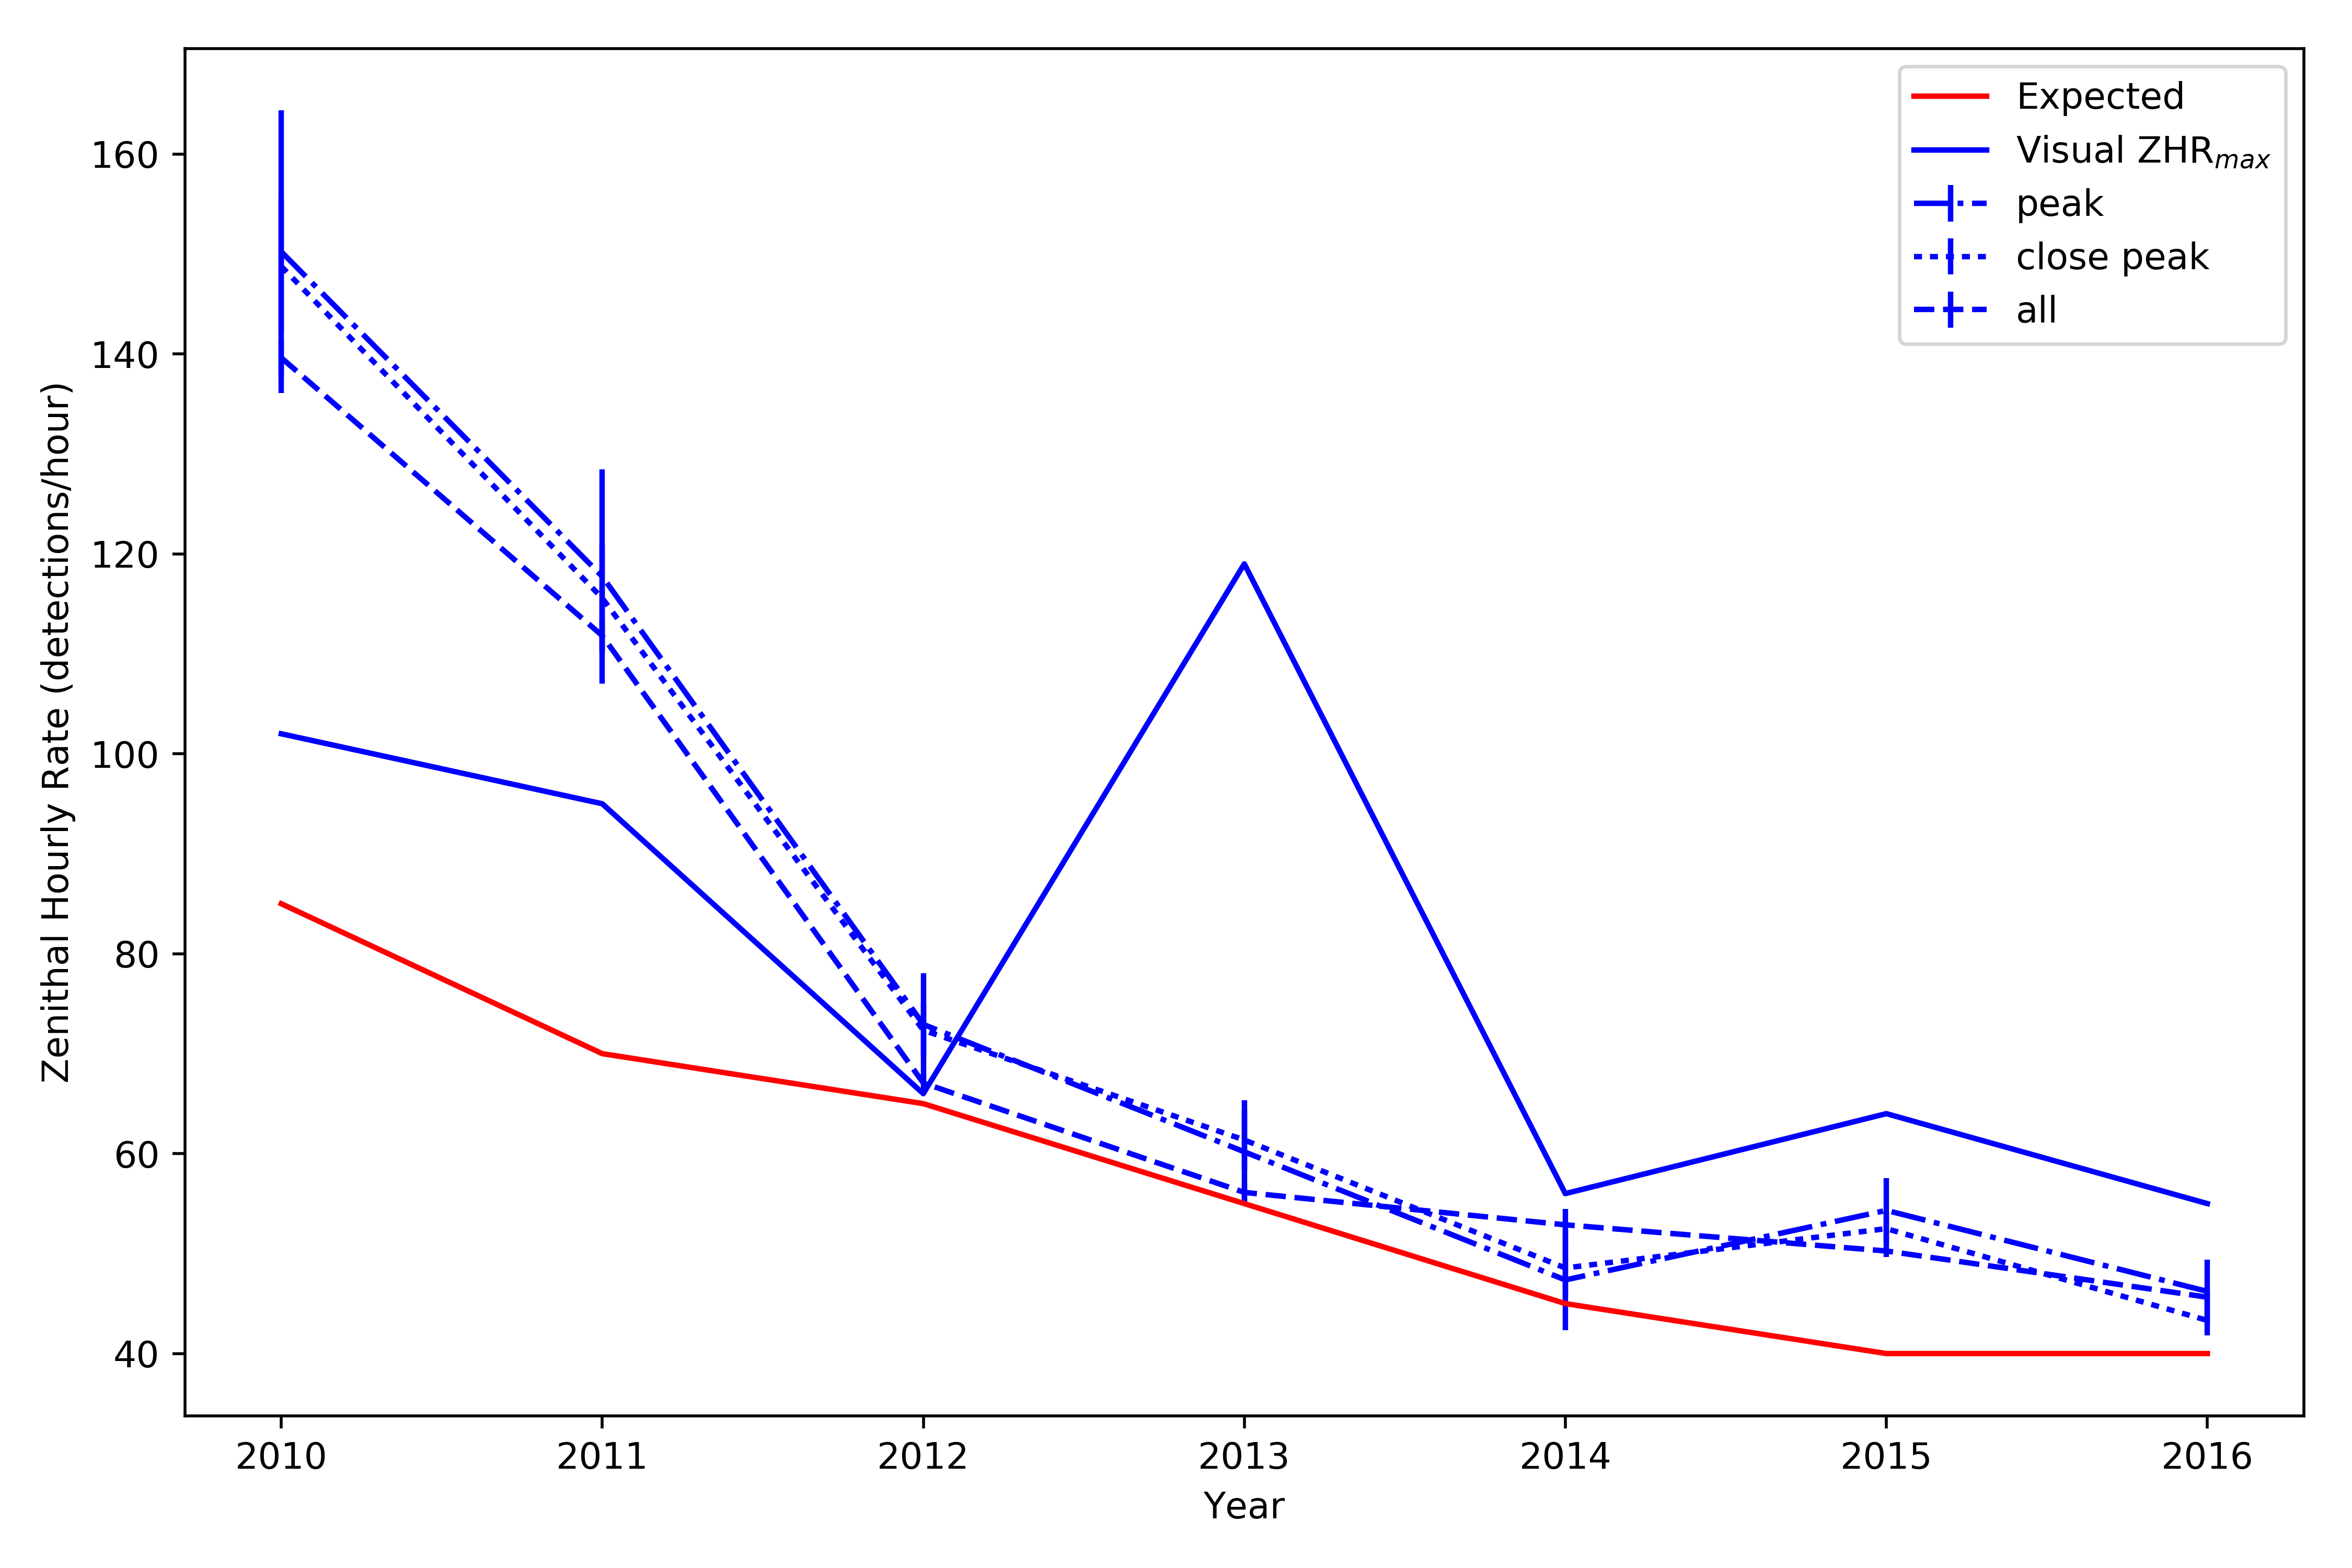
\includegraphics[width=\linewidth]{zhr/eta_aquariids_notitle}
	\caption{$\eta$-aquariids shower mean radio ZHR compared to visual maximum
	ZHR and expected ZHR.} 
	\label{fig:zhr:eaq}	
\end{figure}

The radio ZHR results are of very similar value to the maximum visual ZHR for
each year. Year on year changes are reflected well by the radio results, though
the standard errors are relatively large. This could be due to a low sample
size, or simply disagreements between observers in the sample. However, the
mean values correlate well with visual ZHR.

\paragraph{Correlation}

It is difficult to comment on how good the correlation is when taking into
account all the previous results, so it is best to use a scatter graph of all
results. Figure~\ref{fig:zhr:corr1} demonstrates the correlation between visual
and radio ZHR. The dotted line shows the line of best fit. It is clear from this
figure that there is a correlation between radio and visual ZHR results. There
are some anomalous results, but this is expected from any dataset. The
correlation coefficient is $r = 0.458444$, with p-value of $p = 0.00175$,
indicating there is a good correlation.

\begin{figure}
	\centering
	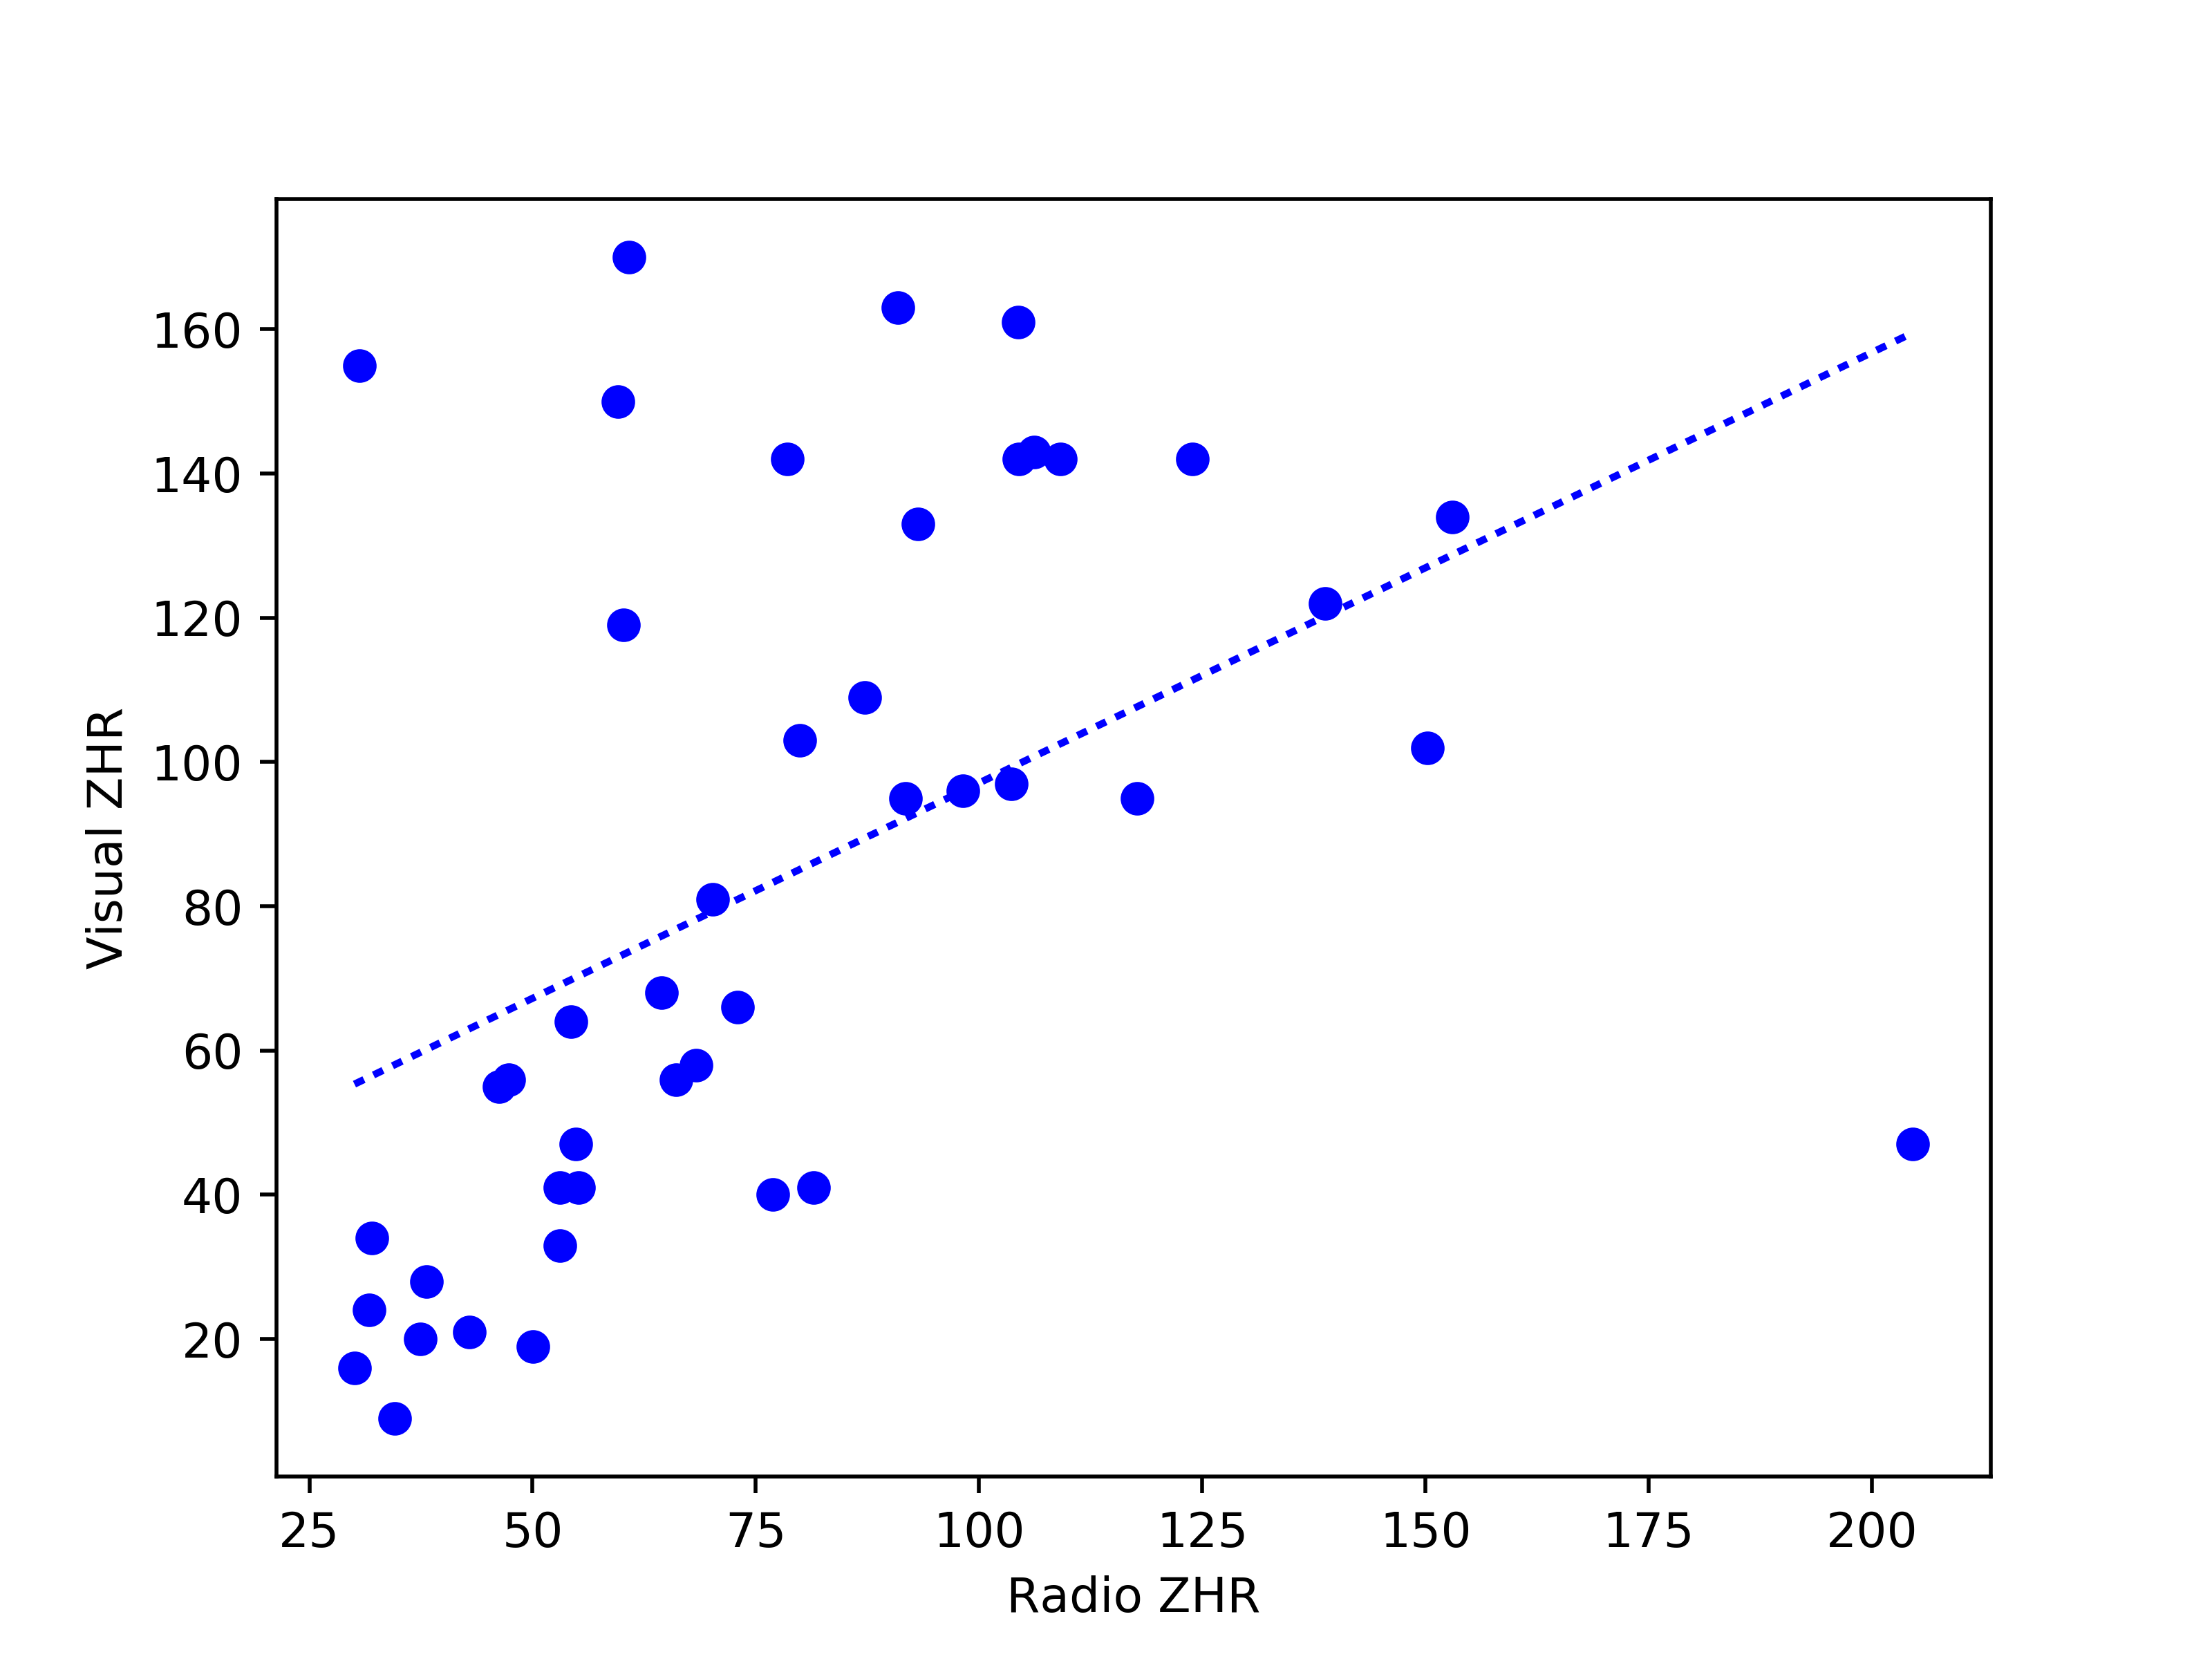
\includegraphics[width=\linewidth]{zhr/peak_scatter}
	\caption{Scatter graph of visual and radio ZHR results. Visual ZHR is the
	maximum visual ZHR of the peak period, radio results are the mean ZHR of the
	peak period.}
	\label{fig:zhr:corr1}
\end{figure}

\subsection{Correction factors} 
The results for the correction factors are shown in table~\ref{tab:corfac}.
There is no field of view factor for the Leonids shower since there were no
values larger than 0. Equally the Orionids field of view factor can be
disregarded since the standard error is larger than the mean itself.

\begin{table} 
	\begin{tabular}{c r@{ \,$\pm$\, }l r@{ \,$\pm$\, }l} 
		\hline
		Shower & m & S.E. & k & S.E.\\ \hline 
		Geminids & 6.63 & 1.00 & 0.418 & 0.0334 \\ 
		Leonids & 7.29 & 0.0563 & 0 & 0 \\ 
		Orionids & 6.96 & 0.0382 & 0.0581 & 1 \\ 
		Perseids & 6.69 & 0.0157 & 0.267 & 0.0500 \\ 
		Quadrantids & 6.56 & 0.0209 & 0.214 & 0.0140 \\ 
		$\eta$ aquariids & 6.77 & 0.0551 & 0.240 & 0.0424 \\ \hline 
	 \end{tabular} 
	 \caption{Limiting magnitude ($m$) and \% obstruction ($k$) for each shower} 
	 \label{tab:corfac} 
\end{table}

\section{Discussion}

\subsection{Comparison}

\paragraph{Peak\\}

Frequently throughout the data the mean ZHR for the period of the peak is lower
than the peak $\pm$ 2 days. This indicates that the peak is in fact different
to that used for calculating the ZHR. Alternatively, this could be due to a
difference in the size of density throughout the meteor stream that causes each
meteor shower. As the Earth moves through the stream, there may be smaller
debris causing the shower, which would not be as easily noticed in visual
meteor detection, but with radio detection's greater effective limiting
magnitude, this is noticeable. This may also explain why in some showers, in
some years, the  mean ZHR decreases from the entire active range towards the
peak, whereas some simply decrease for the peak compared to the peak $\pm$ 2
days, but the mean ZHR for the peak is still greater than the entire active
range. 

In some results, there is a large increase from the peak $\pm$ 2 days to the
peak period. This indicates a shower with an intense peak, where the stream
density increases dramatically on the peak day. The exhibition of this in the
radio ZHR results indicate that it is a good measure of activity in a shower and
can yield useful information.

Provided the data was adequate, it may be possible to estimate the true
peak of a meteor shower. Analysing the mean, or 90th percentile, of the ZHR for
a range of 24 hour periods, and selecting the largest values, should indicate
which period contained the peak. This could, of course, then be focused down
into 1 hour periods.

\paragraph{Stream density\\}

In the geminid shower especially, there is not a large amount of variation
between each period for each respective year. This indicates that the debris
density of the stream is more consistent than most streams. In the quadrantids
shower, the opposite occurs. The variation between the peak and other periods
is significant and this indicates that the stream density changes much more on
the peak.

\paragraph{Variation correlation\\}

In most showers, the variation in the maximum visual ZHR is reflected in the
calculated mean ZHRs. The trends in visual ZHR are reflected well by the radio
results. This suggests that the formula used to calculate the data works well
and is valid as a method of analysing shower activity using radio meteor
detection.  However, the difference between the maximum visual ZHRs and the
means is still significant for some showers, indicating that other correction
factors such as field of view and limiting magnitude still have an impact. The
maximum visual ZHR is a better indicator for this variation than the expected
ZHR, since the expected ZHR is only an estimate, whilst the maximum visual ZHR
is a direct calculation from recorded data. The good correlatoin is supported by
the result of $r = 0.458444$ and p-value indicating that, at the $1\%$
significance level, there is a good correlation.

\subsection{Correction factors}

\subsubsection{Field of view}

The values for $k$ are used to calculate the field of view correction factor.
The values are not as expected. Typically, 50\% or less of the sky can be seen
with any normal sized (< 5m) receiver. For example, see
figure~\ref{fig:zhr:beam} which shows the beam of a Yagi antenna. Clearly, the
results do not agree with this beam, much more than 40\% of the view is not
seen. (I use a yagi antenna as an example since it is the most popular antenna
type). The closest value to 50 \% is for the geminids shower, however this is
still not close. It should be noted that this is an estimation: in conjunction
with other factors, values may be closer to expected.  

\begin{figure}[h!]
	\centering 
	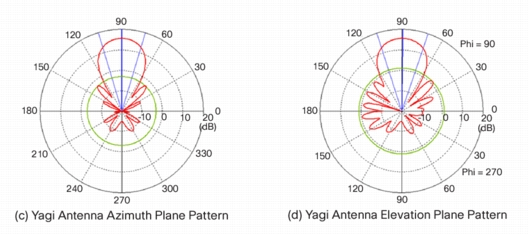
\includegraphics[width=\linewidth]{zhr/yagi} 
	\caption{Yagi beam diagrams \cite{yagi} \label{fig:zhr:beam}} 
\end{figure}

\subsubsection{Limiting magnitude}

The limiting magnitudes are not as high as expected for radio detection. This
demonstrates the fact that this is an estimation --- each factor is calculated
assuming that it is the only factor to be considered, but this is not the case.
The value for $k$ would typically be around 0.5, which would dramatically
increase the ZHR, giving a more accurate value for the limiting magnitude.

\subsection{Formula improvements}

\paragraph{Radiant height correction\\}

An invaluable analysis would be a validation of my proposed method of
calculating the radiant height correction factor. Plotting the relative meteor
flux against the radiant height may reveal a better approximation to the
correction factor. The issue arises in isolating variables such as the actual
ZHR (which may be lower than another time of measurement) and other factors,
such as changing conditions. This can largely be solved by normalizing data
against the expected ZHR, or measuring these changing variables and making a
comparison.

\paragraph{Diurnal shift correction\\}

The diurnal shift of an observation can often be extreme, with a large range of
variation over the course of 24 hours. Estimating this diurnal shift using
techniques from chapter~\ref{chap:diurnalshift} will give an optimal fit sine
curve, from which the expected number of meteors detected from this diurnal
shift can be calculated. This will then replace the background detection count
and will provide a more accurate estimate of the ZHR.

\paragraph{Limiting magnitude\\}

The limiting magnitude for a radio antenna is difficult to calculate. The only
practical way to work it out is to estimate based on what the antenna can be
pick up. Knowing this will refine the formula further, since an accurate
estimate of the limiting magnitude allows the population index to be utilised
which is an important factor.

\paragraph{Field of view\\}

There are techniques to estimate the field of view available to a radio
antenna. If this is done, then the formula can be improved simply by
multiplying by the factor $F$ where $F = \frac{1}{1-k}$.

\subsection{Inaccuracies}

\subsubsection{Re-entry direction}

The radio detection of a meteor largely depends on the direction it is
travelling. A meteor is best detected when travelling directly across the
``field of view'' of the receiving antenna. It is difficult to take this into
account when calculating the ZHR, but the general direction in which meteors
are travelling from the radiant will have an effect on this value.

\subsubsection{Observing station vs. transmitting antenna}

There is often a marked difference between the location of the transmitting
antenna and the receiving antenna, where the data is recorded. This results in
a potentially large inaccuracy since the radiant altitude and other factors at
the receiving station may be very different to the transmitting station.

\subsubsection{Antenna type}

When calculating the limiting magnitude and field of view, the type of antenna
will influence the results greatly. Certain antennas may have a much larger
field of view, or be less sensitive and have a lower limiting magnitude. 

\section{Conclusion}

The ZHR formula, with modification, is valid for use in radio meteor detection.
This is apparent from the good correlation between ZHR results from radio
observation data when compared with visual observation, up to a constant
offset. With knowledge of an antenna's field of view, and the population index
of a meteor shower, estimations can be made more accurately. Further study is
required to analyse the distribution of meteor magnitudes for larger limiting
magnitudes than 6.5, as well as the best way to estimate the background
detection rate of an observation station. Analysis of ZHR is difficult, given
the number of factors involve, and how difficult it is to isolate these
factors, such as field of view.
